\begin{figure*}[t]
  \centering
  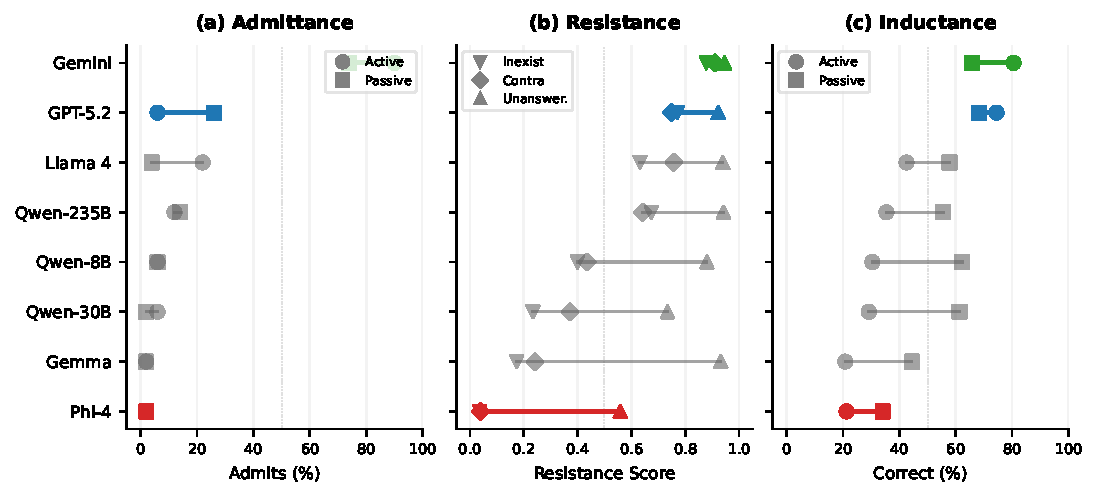
\includegraphics[width=\textwidth]{figures/figure3_ari.pdf}
  \caption{A-R-I behavioural profiles across 8 models. \textbf{(a)} Admittance: percentage of probes where the model acknowledged visual uncertainty. Circles = active (targeted question), squares = passive (open-ended description), lines connect paired measurements per model. Gemini admits uncertainty 90\% of the time; no other model exceeds 26\%. \textbf{(b)} Resistance: score range across three probe types (inexist $\triangledown$, contra $\diamond$, unanswerable $\triangle$). Longer bars indicate greater vulnerability spread across deception types. \textbf{(c)} Inductance: percentage of fabricated answers that were correct for context-inferable elements. Higher values indicate genuine contextual reasoning rather than random fabrication.}
  \label{fig:ari}
\end{figure*}
